%%%%%%%%%%%%%%%%%%%%%%%%%%%%%%%%%%%%%%%%%
% University/School Laboratory Report
% LaTeX Template
% Version 3.0 (4/2/13)
%
% This template has been downloaded from:
% http://www.LaTeXTemplates.com
%
% Original author:
% Linux and Unix Users Group at Virginia Tech Wiki 
% (https://vtluug.org/wiki/Example_LaTeX_chem_lab_report)
%
% License:
% CC BY-NC-SA 3.0 (http://creativecommons.org/licenses/by-nc-sa/3.0/)
%
%%%%%%%%%%%%%%%%%%%%%%%%%%%%%%%%%%%%%%%%%

%----------------------------------------------------------------------------------------
%	PACKAGES AND DOCUMENT CONFIGURATIONS
%----------------------------------------------------------------------------------------

\documentclass{article}
\usepackage[utf8]{inputenc}
\usepackage{polski}
\usepackage[polish]{babel}
\usepackage{cite}
\usepackage{url}
\usepackage{pdfpages}


\usepackage{graphicx} % Required for the inclusion of images

\setlength\parindent{0pt} % Removes all indentation from paragraphs

%\renewcommand{\labelenumi}{\alph{enumi}.} % Make numbering in the enumerate environment by letter rather than number (e.g. section 6)

%\usepackage{times} % Uncomment to use the Times New Roman font

%----------------------------------------------------------------------------------------
%	DOCUMENT INFORMATION
%----------------------------------------------------------------------------------------

\title{Modelowanie zawodów Formuły 1} % Title

\author{Sabina \textsc{Rydzek} \\ Mateusz \textsc{Kotlarz} \\ Kacper \textsc{Furmański}} % Author name

\date{\today} % Date for the report

\begin{document}

\maketitle % Insert the title, author and date


\begin{abstract}
Projekt ten obejmuje stworzenie modelu wyścigu Formuły 1 oraz jego symulację na wczytanym przez użytkownika torze. Wykorzystuje automaty komórkowe. Symulowane są różne czynniki i typy nawierzchni mające wpływ na trasę i sposób jazdy bolidów. Zamodelowane zostały umiejętności kierowców, które mają wpływ na styl ich jazdy oraz umiejętność przewidywania oraz osiągi. Statystyki umożliwiają odczyt prędkości poszczególnych bolidów oraz ich pozycję na mecie. Projekt jest otwarty i umożliwia tworzenie i wczytywanie innych tras w odpowiednim formacie.
\end{abstract}

\pagebreak

%----------------------------------------------------------------------------------------
%SECTION 1
%----------------------------------------------------------------------------------------

\section{Formuła 1}
Formuła 1 (Grand Prix) to cykl międzynarodowych wyścigów samochodowych. Samochody, biorące udział w wyścigach nazywane są bolidami. Mają charakterystyczny kształt, który pozwala na uzyskanie bardzo dużej przyczepności. Samochody potrafią uzyskać bardzo dobre osiągi i prędkości powyżej $300$ km/h w mniej niż 9 sekund. \\

Wykorzystany przez nas tor to Silverstone położony w Wielkiej Brytanii \cite{track}. Ma długość $5,891$ km.

\begin{figure}[h]
\begin{center}
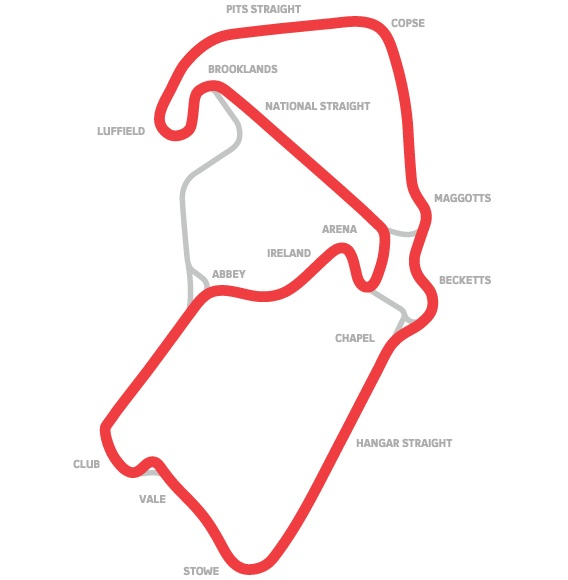
\includegraphics[scale=0.4]{silv.jpg}
\caption{Tor Silverstone}
\end{center}
\end{figure}

\section{Założenia projektu}
\begin{itemize}
\item Użycie do modelowania automatów komórkowych
\item Przeniesienie obrazu trasy wyścigu na dwuwymiarową siatkę
\item Zamodelowanie ruchu samochodów po trasie na siatce
\item Zamodelowanie zachowania się kierowców na drodze
\item Wprowadzenie współczynników zmieniających zachowanie się samochodów i kierowców
\end{itemize}

\section{State of the Art}
Zagadnienie symulacji wyścigów F1 jest bardzo złożone. Niestety, do wielu studenckich prac dotyczących tego tematu nie ma pełnego dostępu.  \\

Z symulacją F1 na University of Cambridge zmierzył się Robert Woolley \cite{woolley}, który dopasował istniejące programy do symulacji wyścigów na potrzeby F1 tak, by były one użyteczne dla FIA (Fédération Internationale de l'Automobile). \\

Jednym z programów pozwalających na symulację wyścigów jest RaceSim \cite{race}, który po wprowadzeniu danych samochodu oraz trasy 3D potrafi wyznaczać współczynniki przyczepności, drogę hamowania itp. oraz reprezentować dane graficznie.  jest to jednak bardziej symulacja fizyki samochodu, niż jego zachowania się na torze. \\

Jednym z ciekawszych podejść do tematu symulowania wyścigów F1 za pomocą automatów komórkowych jest GCA - Global Cellular Automata, które rozszerzają definicję sąsiedztwa i określają je dynamicznie, a nie jak w definicji klasycznej statycznie \cite{gca}. Opiera się on również na znanym algorytmie symulacji samochodów.

\begin{center}
\begin{figure}[h]
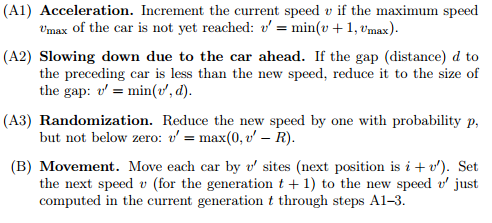
\includegraphics[scale=0.9]{alg.png}
\caption{A cellular automaton model for freeway traffic}
\end{figure}
\end{center}

Podejście GCA upraszcza model, ponieważ w chwili $t$, automat wie już, gdzie będzie znajdował się w chwili $t+1$. Wie dokładnie, na których komórkach znajdują się samochody przed nim i za nim. Niestety przy próbie modelowania samochodów w trakcie wyścigu, sprawa się komplikuje, ponieważ listę z dołączeniami, na której oparty jest algorytm, trzeba rozszerzać i dopisywać kolejne warunki. \\

W pracy Hoffmanna i Margensterna \cite{maurice} opisane jest podejście do algorytmu wyznaczania trasy przez jadący samochód. Na drodze ustawianie są punkty, które są dla pojazdu tymczasowymi celami, które stara się osiągnąć. Na każdym odcinku przyspiesza, a później hamuje. Pozwala to jednak na płynne przemieszczanie się samochodu po torze bez obijania się o barierki.


\section{Automaty komórkowe}

W projekcie zastosowany jest model automatów komórkowych. Jest to dyskretny, nieliniowy model, który składa się ze skończonej oraz uporządkowanej liczby \textit{komórek}, które w każdej chwili posiadają swój z góry określony stan, który wyznaczany jest na podstawie komórek sąsiadujących (wg. wybranego sąsiedztwa). \\

Wg klasycznej definicji, automat komórkowy to trójka (L,S,f), gdzie:
\begin{itemize}
\item L - siatka komórek przestrzeni n-wymiarowej
\item S - zbiór stanów pojedynczej komórki
\item f - reguła określająca stan komórki w chwili $t+1$ w zależności od stanu danej komórki i komórek sąsiednich w chwili $t$.

$$
s_{i}(t+1) = f(s_{j}(t)), j \in O(i)
$$

gdzie $O(i)$ to otoczenie komórki
\end{itemize}

Takie podejście pozwala wyeliminować nadmiarowe obliczenia oraz potrzebę śledzenia pozycji. Dodatkowo, pozwala na dodatkowe optymalizacje przy wykorzystaniu programowania równoległego \cite{cellularAutomata}. \\


\subsection{Czas}
Automaty komórkowe nie działają w \textit{czasie rzeczywistym}. Zmiana czasu to stworzenie nowej generacji komórek na podstawie określonych reguł ich zachowania \cite{nature}.


\subsection{Stany}

Najprostsze automaty komórkowe posiadają tylko dwa stany - jak np. w Game of Life, gdzie komórka jest żywa (1) lub martwa (0) \cite{kulak}. Zbiór stanów zazwyczaj jest taki sam dla każdej komórki. 

	
%----------------------------------------------------------------------------------------
% SEKCJE DOKUMENTACJI
%----------------------------------------------------------------------------------------
\section{Pojęcia podstawowe i opis rozwiązań}
\subsection{Reprezentacja bolidu}
Bolid reprezentowany jest przez środek ciężkości znajdujący się w jednej komórce i nakładkę, która zajmuje pół komórki z przodu i pół komórki z tyłu bolidu.

\subsection{Komórki}
\begin{itemize}
\item SurfaceType - ROAD, GRASS, WORSE ROAD, BARRIER, START LINE, SAND - określają typ nawierzchni oraz przypisane im współczynniki, które wpływają m.in. na szybkość, przyczepność bolidów. 
\item Direction -  NONE, TOP LEFT, TOP, TOP RIGHT, LEFT, RIGHT, BOTTOM LEFT, BOTTOM, BOTTOM RIGHT; - określają kierunki, w których może poruszać się bolid, z tych wybierane są te, na które pozwala orientacja bolidu, trasa oraz reguły. Określany jest tutaj również kąt położenia nakładki bolidu na siatce
\end{itemize}

Komórka w algorytmie może posiadać swój stan - jest/nie ma samochodu. Ograniczona jest również możliwa do rozwinięcia prędkość do $302$ km/h. \\

Direction jest cechą pozwalającą kierowcy ocenić, kiedy należy hamować, przyspieszać, przygotowywać się do zakrętu. Model przyjmuje założenie, że kierowcy znają trasę, po której jadą, dlatego kierunki określane są na trasie tak samo dla każdego samochodu.

\subsection{Sąsiedztwo}
Podstawowym sąsiedztwem dla komórki jest sąsiedztwo Moore'a. Na decyzję kierowcy wpływają jednak również bolidy, które znajdują się w zasięgu DRIVER VISIBILITY

\section{Modelowanie ruchu bolidów}
Projektowanie modelu ruchu bolidów oparliśmy na rozwiązaniu przedstawionym w pracy \textit{Social Distances} \cite{was}. Samochód reprezentowany jest przez prostokąt o środku znajdującym się w środku jednej z komórek. Bok komórki to $2,6 m$ w rzeczywistości, dlatego modelowane przez nas bolidy mają długość $5,2 m$.

Samochód może poruszać się w 8 kierunkach, z których każdy jest odpowiednim kątem obrotu (wielokrotności $45^{\circ}$) prostokąta będącego naszym bolidem. Przejazd bolidu na sąsiednią, odpowiednią komórkę zależny jest od orientacji bolidów w przestrzeni (czyli położenia reprezentujących je prostokątów). Bolidy starają się unikać kolizji, dlatego jeżeli konfiguracja uznana jest za niebezpieczną, bolid może zwolnić, przyspieszyć, bądź spróbować zmienić swoją orientację. Oczywiście, jeżeli nie będzie to możliwe, na co mogą wypływać odpowiednie współczynniki przyczepności albo umiejętności kierowców, nastąpi zderzenie i bolidy odpadną z wyścigu.   \\

\subsection{Skalowanie}
Dużym problemem jest skalowanie, ponieważ tory są bardzo duże w stosunku do wielkości bolidu. Aplikacja posiada możliwość przybliżania i oddalania widoku siatki oraz opcję podążania za wybranym samochodem.

\begin{figure}[h]
\begin{center}
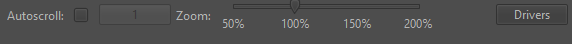
\includegraphics[scale=0.8]{scroll.png}
\caption{Opcja przybliżania, autoscroll}
\end{center}
\end{figure}


\subsection{Poruszanie się}
Orientacja bolidu zmieniana jest w trakcie poruszania się do kolejnej komórki.


\section{Dane wejściowe i wyjściowe}
Wejścia systemu to:
\begin{itemize}
\item kierowcy (imię, nazwisko, poziom umiejętności)
\item trasa przejazdu
\item współczynniki (wprowadzone domyślne, bądź przez użytkownika)
\item pozycja startowa bolidów
\end{itemize}

Wyjścia systemu to:
\begin{itemize}
\item wyniki (pozycje kierowców)
\item wyliczone przyspieszenie, prędkość
\item czas najlepszego okrążenie
\item czas bieżącego okrążenia
\end{itemize}


\section{Automaty komórkowe - zastosowanie w projekcie}
\subsection{Siatka komórek}
Tor F1 oraz jego otoczenie jest tablicą komórek o różnych współczynnikach w zależności od ich typu (trawa, piasek, asfalt itp.). Głównym problemem w zastosowaniu modelu automatów komórkowych jest to, że bolid jako ciało stałe zajmuje więcej niż jedną komórkę. Oddziaływanie na siebie wielu \textit{bloków} komórek kłóci się z podstawowym założeniem, że w obliczeniach pod uwagę brane są tylko komórki w określonym sąsiedztwie \cite{particleSimulation}. Aby poradzić sobie z tym problemem, bolid przedstawiony jest tylko jako środek ciężkości (jego obrzeża są nakładką na torze). 	\\

Na przedstawienie toru jako tablicy złożonej z komórek odpowiedniego typu pozwala TrackEditor. Część potrzebnych  skryptów wykonana została w środowisku Matlab. \\

Do toru ręcznie dodany jest punkt startowy oraz ustawione na starcie bolidy.

\subsection{Stany komórek}
W komórce może znajdować się środek ciężkości samochodu (1), bądź nie (0).

\subsection{Reguły}
\subsubsection{Podstawowe kroki algorytmu}
\begin{enumerate}
\item Sprawdzanie, kiedy nastąpi kolizja
\item Przeliczanie drogi oraz prędkości, ewentualna aktywacja KERS
\item Element losowości - dołączany element błędu kierowcy
\item Sprawdzanie możliwych komórek, na które samochód może przejechać oraz dystansu od przeciwników przed bolidem
\item Obliczanie nowej prędkości
\item Określenie przesunięcia samochodu wraz z nowymi współczynnikami
\end{enumerate}

\subsubsection{Sprawdzanie kolizji}
Jeżeli w sąsiedztwie bolidu znajduje się inny bolid, którego kąt różni się od kąta wyliczanej komórki, wtedy następuje kolizja.

\subsubsection{Przeliczanie drogi, prędkości, wyliczanie przyspieszenia}
Wartości współczynników wyliczone zostały ze wzorów:
$$
s = s_{0} + v_{0}t + \frac{at^{2}}{2}
$$
$$
v = v_{0} + at
$$

\subsubsection{Element losowy - błędy kierowców}
Każdy kierowca ma przypisany poziom umiejętności. Są to MONKEY, NOVICE, INTERMEDIATE, PRO, EXPERT, MASTER, w rosnącej kolejności. W zależności od poziomu, odejmowane są odpowiednie współczynniki do przyspieszenia (utrzymanie przyczepności na torze) oraz liczona możliwość popełnienia przez niego błędu w ocenie sytuacji, wyboru odpowiedniego kierunku.

\subsubsection{Driver visibility}
Driver visibility to przestrzeń, która ma wpływ na zachowanie kierowcy. Jest w postaci trójkątnej, rozszerzająca się od bolidu. Na jej podstawie wyliczany jest kierunek, do którego obrania próbuje dążyć kierowca. Wyliczana jest mediana z każdego rzędu komórek, a następnie z tego uzyskiwana średnia. Wygląd przestrzeni zmienia się w zależności od kąta położenia bolidu.\\

\begin{figure}[h]
\begin{center}
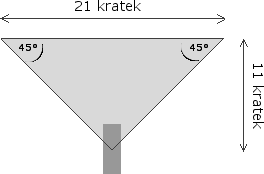
\includegraphics[scale=0.6]{visibility-top.png}
\caption{Driver visibility dla wielokrotności kąta $90^{\circ}$}
\end{center}
\end{figure}

\begin{figure}[h]
\begin{center}
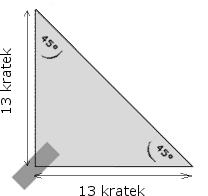
\includegraphics[scale=0.6]{visibility-top-left.png}
\caption{Driver visibility dla kątów $k+45^{\circ}$}
\end{center}
\end{figure}

Jeżeli w zasięgu wzroku i na trasie kierowcy znajdzie się rywal, bolid stara się uniknąć kolizji i przyhamowuje. Wpływ na hamowanie ma poziom umiejętności kierowcy i wyliczony wcześniej współczynnik - jeżeli kierowca zahamuje za późno lub z zza dużej prędkości, kolizji nie uda się uniknąć.

Jeżeli w przestrzeni przed kierowcą nie znajduje się żaden jego rywal oraz zakręt, a naładowanie KERS osiąga 100\%, kierowca włącza go na następne $6.7 s$.

%Obrazek


\subsubsection{Obliczanie nowych współczynników}

Wartości nowych współczynników wyliczane są za pomocą podanych wcześniej wzorów.

\subsubsection{Przesunięcie samochodu do nowej komórki}
W każdej iteracji wyliczany jest nowy przejechany dystans od ostatniej iteracji. Jeżeli jest on większy niż $2,6 m$, nastąpi przesunięcie samochodu do nowej komórki, jeżeli nie, samochód pozostaje w tej samej komórce a dystans w następnej iteracji dodaje się. Jedna iteracja domyślnie trwa $20 ms$.

Jeżeli prędkość samochodu jest za duża (zbliża się do $300 km/h$), samochód może nie zdążyć wyhamować i nie może od razu zmienić kierunku jazdy, wtedy jest duża szansa, że wypadnie z toru.

\subsubsection{Wyprzedzanie}
Samochody wyprzedzają się z bardzo małym prawdopodobieństwem (podobnie jak w rzeczywistych wyścigach). Jeżeli w sąsiedztwie bolidu znajduje się inny samochód, kierowca stara się wyminąć go z prawej albo lewej strony, obierając właściwy kierunek. 

\subsubsection{Wypadki}
Wypadkiem może być:
\begin{itemize}
\item kolizja - kiedy zderzają się dwa samochody (najczęściej spowodowane gwałtownym hamowaniem)
\item wypadnięcie z trasy - bolid wypada z wyścigu, kiedy utknie na trawie albo piasku, nie ma już żadnego kierunku do obrania (NONE), a jego przyspieszenie jest mniejsze od zera
\item uderzenie w barierę
\end{itemize}

\section{Zakończenie symulacji}
Symulacja nie ma z góry określonych warunków zakończenia. Zakończenie wywoływane jest na życzenie użytkownika.

\pagebreak

\section{Implementacja}
\subsection{Wybór języka}
Algorytm zaimplementowany będzie przy użyciu języka programowania Java, który twórcy projektu znali najlepiej. Podejście obiektowe pozwala na jasne i przejrzyste przedstawienie algorytmu. Szybkość działania pozwala na stosunkowo płynną animację poruszania się samochodów na torze. Java pozwala również na korzystanie z aplikacji na innych platformach niż Windows (testowane na Windowsie 8.1 64-bit oraz na Fedora 19 64-bit). Siatka komórek jest zmodyfikowaną i zoptymalizowaną siatką używaną na laboratoriach z Symulacji i Sterowania Procesów Dyskretnych. Opis paczek oraz klas wraz z komentarzami dostępny jest jako \textit{JavaDocs}. W projekcie wykorzystane są również dwie biblioteki zewnętrzne - Substance oraz Trident używane do poprawienia wizualnie wyglądu GUI.


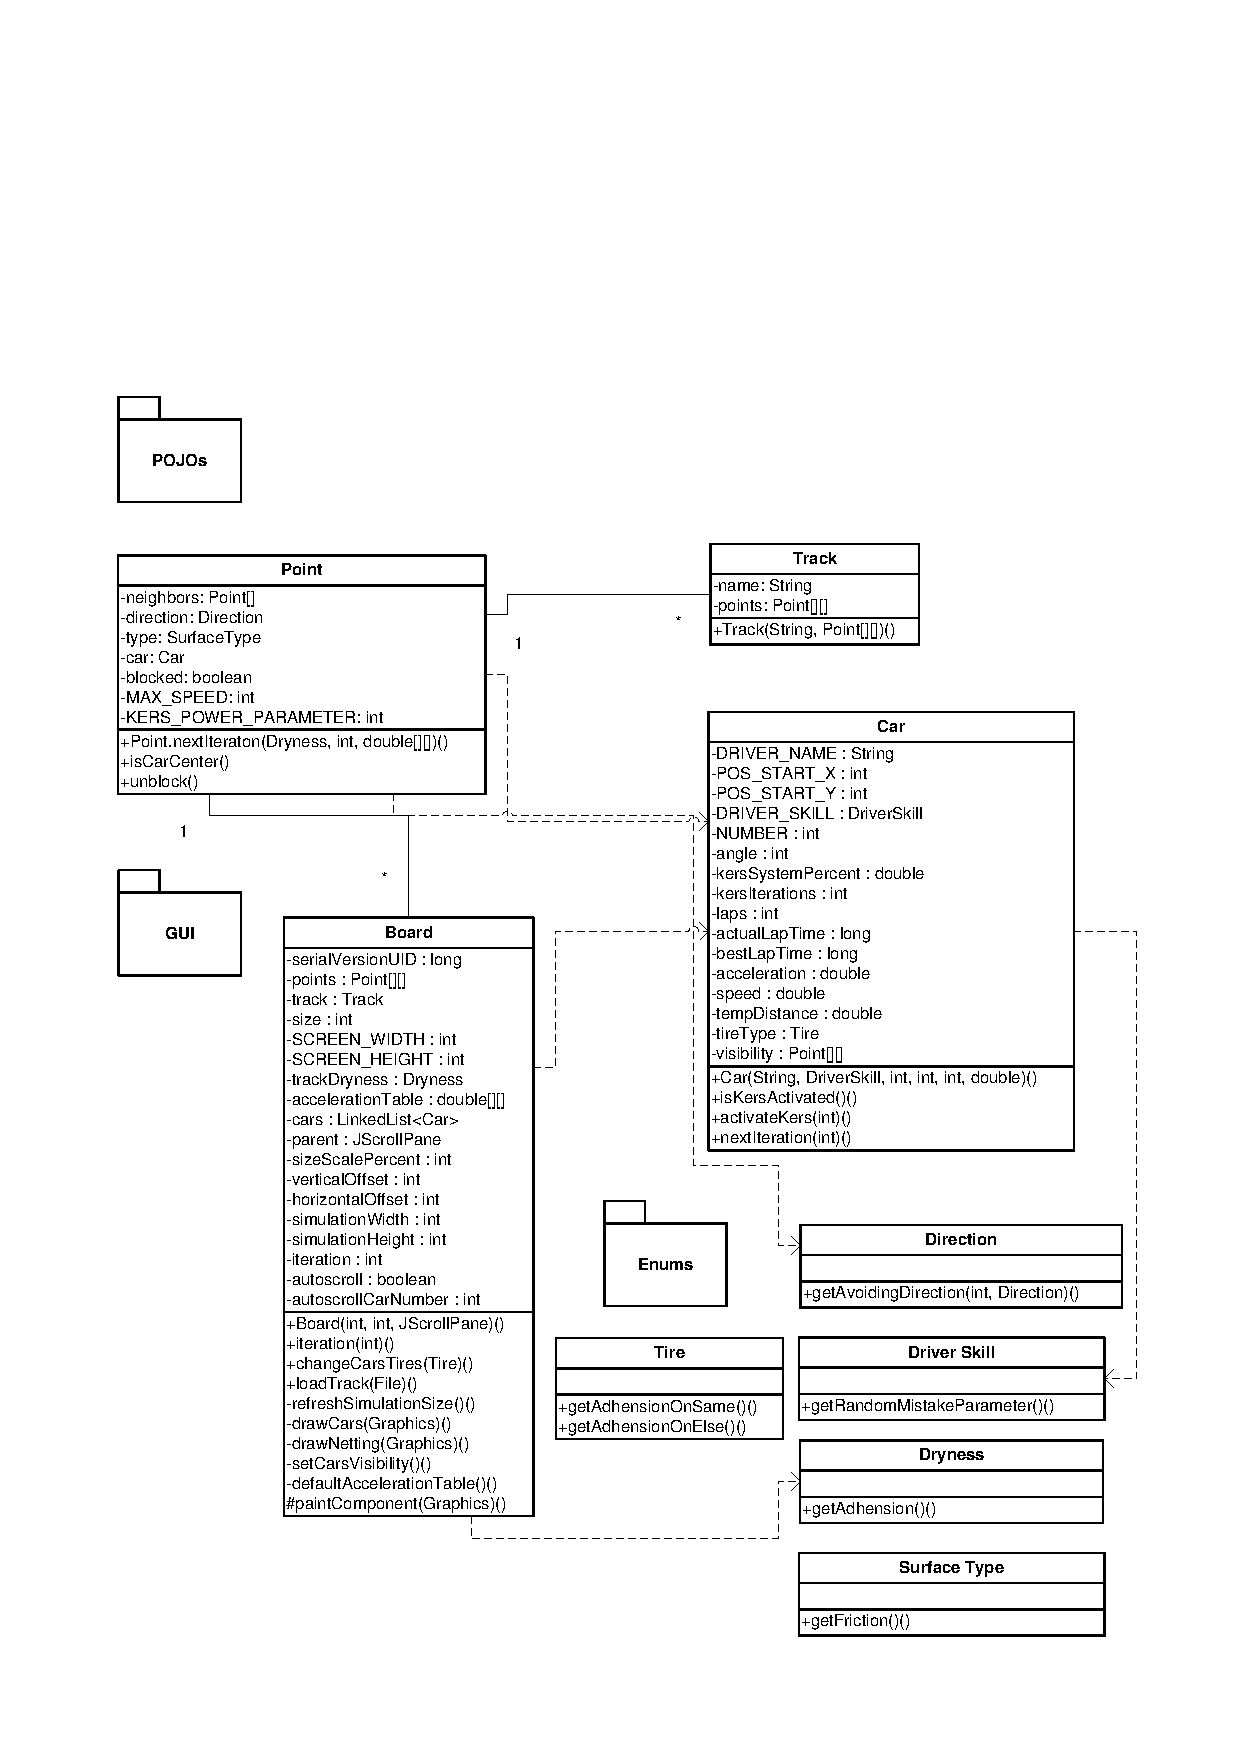
\includepdf[pages=1,pagecommand=\subsection{Diagram UML}Diagram przedstawia wybrane klasy z paczek POJOs GUI oraz Enums. Dla czytelności nie są wyszczególnione settery oraz gettery atrybutów oraz niektóre atrybuty. Pełny opis klas znajduje się w JavaDocs.]{uml.pdf}
\includepdf[pages=2,pagecommand=\subsection{Przypadki użycia dla użytkownika}]{uml.pdf}
\includepdf[pages=3,pagecommand=\subsection{Activity diagram dla pojednynczej komórki}]{uml.pdf}

\subsection{GUI, opcje aplikacji, możliwości doboru współczynników}
Po starcie programu uruchamia się okno do wyboru trasy. Trasy mogą być tworzone z wykorzystaniem Track Editor i mają rozszerzenie \begin{verbatim}
.track
\end{verbatim}

Elementy GUI:
\begin{itemize}
\item Load track - pozwala na wczytanie trasy
\item Simulation parameters - otwiera okno z opcjami
\item Start - uruchamia symulację
\item Clear - powraca do stanu początkowego
\item About - o twórcach projektu
\item Exit - wyjście z programu
\item Autoscroll i Zoom - odpowiada za widok	
\item Drivers - otwiera okno ze statystykami
\item Results - otwiera okno z wynikami
\end{itemize}

Simulation speed wpływa na przedstawienie na symulacji jednej sekundy (np. $2x$ oznacza, że jedna sekunda symulacji to $0.5s$ w rzeczywistości. \\
Iteration delay odpowiada za to, jak wiele iteracji przypada na jedną sekundę. \\
Refreshing odpowiada za tempo odświeżania tabeli wyników i statystyk.\\

Współczynniki Gas, Brake i None określają wartość przyspieszenia (hamowania) w różnych zakresach prędkości samochodu.\\
\pagebreak
\begin{figure}[h]
\begin{center}
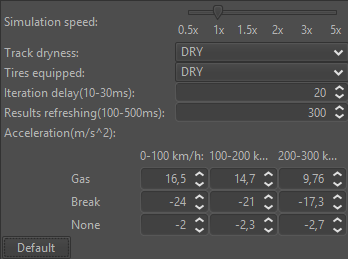
\includegraphics[scale=0.8]{options.png}
\caption{Możliwości wpływu na symulację}
\end{center}
\end{figure}


\section{Wyniki symulacji}
\subsection{Przykładowe uzyskane wyniki i statystyki}

\begin{figure}[h]
\begin{center}
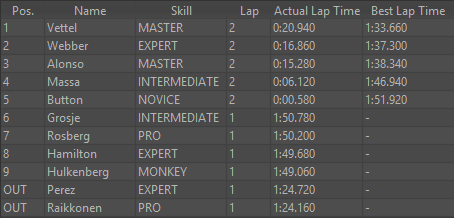
\includegraphics[scale=0.8]{results.png}
\caption{Przykładowe wyniki po pierwszym okrążeniu na nawierzchni suchej (opony DRY)}
\end{center}
\end{figure}

\pagebreak

\begin{figure}[h]
\begin{center}
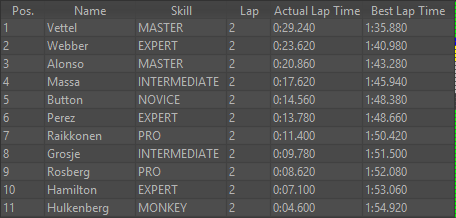
\includegraphics[scale=0.8]{wet.png}
\caption{Przykładowe wyniki po pierwszym okrążeniu na nawierzchni mokrej (opony WET)}
\end{center}
\end{figure}

\begin{figure}[h]
\begin{center}
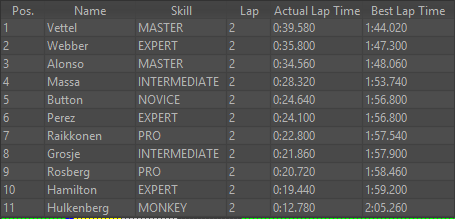
\includegraphics[scale=0.8]{wetdry.png}
\caption{Przykładowe wyniki po pierwszym okrążeniu na nawierzchni mokrej (opony DRY)}
\end{center}
\end{figure}

\begin{figure}[h]
\begin{center}
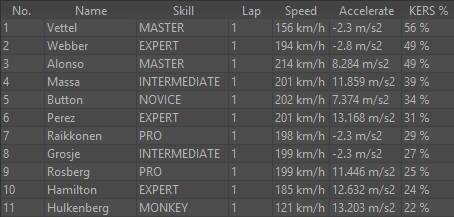
\includegraphics[scale=0.8]{stats.png}
\caption{Przykładowe statystyki}
\end{center}
\end{figure}

Jak widać, wyniki są podobne dla opon suchych na torze suchym i opon WET na torze mokrym. Znacznie się pogarszają, gdy opony nie są przystosowane do nawierzchni. \\

Statystyki na bieżąco pokazują prędkość bolidu, przyspieszenie (hamowanie) oraz poziom naładowania systemu KERS.

\subsection{Kalibracja i walidacja modelu}

Początkowo problemem było takie dopasowanie współczynników, by można było wiernie odwzorować rzeczywisty wyścig na torze. Znając prędkości na zakrętach oraz średnią prędkość na torze, mogliśmy modyfikować współczynniki hamowania, przyspieszenia \cite{track}. Model bierze pod uwagę również przyczepność opon różnego rodzaju na mokrej i suchej nawierzchni. Kalibracja współczynników przyczepności polegała na takim ich dostosowaniu, aby widać było ich wpływ na czas okrążenia oraz umiejętność pokonywania zakrętów. \\

Współczynniki dobieraliśmy sprawdzając czas i ilość kolizji kolejnych okrążeń, na przykład dla suchej nawierzchni i dobranych do niej opon: \\

\begin{tabular}{c|c|c|c}
Test & Kolizje & Najlepszy czas & Najgorszy czas \\
\hline
1 & 1 & $1:35$ & $1:58$ \\
\hline
2 & 2 & $1:30$ & $1:48$ \\
\hline
3 & - & $1:29$ & $1:38$ \\
\end{tabular} \\

Kalibracja współczynników przyspieszania i hamowania jest również dostępna dla użytkownika. Wartości domyślne dobrane zostały korzystając z dostępnych szybkości na zakrętach. Prędkość maksymalna samochodów została w projekcie ograniczona z góry do $302$ km/h, by prędkości mierzone na zakrętach przypominały prędkości rzeczywiste \cite{fanatic}.

Aktywacja KERS trwa tyle samo, ile w rzeczywistości, a jej współczynnik można przeliczyć na dodatkowych $80$ koni mechanicznych.\\

\pagebreak

Rekord toru należy do Webbera i wynosi $1:33.401$. Prędkości samochodów dopasowane są tak, aby wynik najlepszego kierowcy był zbliżony do czasu Webbera. System KERS (Kinetic energy recovery system) wykorzystywany jest najczęściej na najdłuższej prostej toru - Wellington(1034m). \\

Walidację rozpoczął test komponentów programu. Zostało sprawdzone, czy samochody rysują się poprawnie i czy zmiany współczynników faktycznie mają wpływ na zachowanie się bolidów. Testowanie funkcjonalności było sprawdzeniem poprawności algorytmu - m.in. czy samochody prawidłowo odczytują zbliżający się zakręt, czy nie przekraczają dozwolonych prędkości i czy starają się unikać kolizji. Weryfikacja ilościowa projektu potwierdziła, że prędkości osiągane przez kierowców zgadzają się z prędkościami osiąganymi rzeczywiście, a czasy przejazdu odzwierciedlają umiejętności kierowców, co szczególnie widać na ostrych zakrętach.

Weryfikacja ilościowa ukazuje ważny błąd symulacji, którym jest za duża długość bolidu w stosunku do danych rzeczywistych - $5,6m$ w stosunku do $4,58m$. Jest to spowodowane za małą wydajnością komputera, który ma problem z wyliczaniem tak małych oczek siatki.


\section{Wnioski}
\subsection{Problemy powstałe przy tworzeniu modelu}
Pierwsze problemy pojawiły się już na etapie wybierania podejścia do modelowania tematu za pomocą automatów komórkowych. Zarówno prosta siatka, jak i siatka, której komórki mają inny kształt na zakrętach, miały swoje zalety i wady. Wyzwaniem było również takie zamodelowanie samochodów, które umożliwiało traktowanie go jak pojedynczej komórki. \\

Największym problemem była jednak mocno ograniczona przestrzeń, na podstawie której kierowca może podejmować decyzję. Rozszerzanie sąsiedztwa, albo powiększanie driver visibility znacznie wydłużało czas obliczeń i animacja samochodów przestawała być płynna. \\

Ostatnim z problemów była ograniczona możliwość walidacji modelu. Informacje o ważnych dla symulacji zmiennych są trudnodostępne, a wyliczanie dokładnych współczynników tarcia, przyczepności albo oporu powietrza jest już dziedziną fizyki, z którą twórcy projektu mają małą styczność. 

\subsection{Usytuowanie modelu na tle innych rozwiązań}
Bardzo dużym utrudnieniem był fakt, że podobna symulacja nie jest dostępna, a literatura w dużej mierze dotyczy samego poruszania się samochodów, bądź wyścigów, które nie są tak specyficzne, jak F1. \\

Pomimo dostępnej i omówionej wcześniej literatury (\cite{gca} \cite{race} \cite{was}), twórcy projektu nie mogli skorzystać z przedstawionych tam rozwiązań i technik. Poziom skomplikowania symulacji wymuszał rozszerzenie sąsiedztwa, dodawanie kolejnych instrukcji algorytmu. Dodatkowo ciągłą uwagę należało zwracać na płynność symulacji. \\

W przeciwieństwie do projektu Roberta Woolleya \cite{woolley}, ten model nie wykorzystuje tak skomplikowanej fizyki, dlatego nie może być używany w celach badawczych, choć takie jego przystosowanie jest ważnym kierunkiem jego rozwoju.

\subsection{Sukcesy}
Twórcom udało się osiągnąć równowagę pomiędzy dokładnością obliczeń i szybkością ich wykonywania. Zoptymalizowana siatka pozwoliła na szybsze jej rysowanie i też znacząco zredukowała czas wykonywania kroku symulacji. \\

Jednym z ważnych elementów projektu jest także przyjazne dla użytkownika GUI, które pozwala na ustawianie współczynników, podgląd wyników i statystyk. 

\subsection{Future works - kierunki rozwoju symulacji}
\begin{itemize}
\item możliwość wyboru opon dla konkretnego kierowcy
\item poprawa umiejętności wyboru idealnej trasy przez kierowców
\item zamodelowanie pitstopu
\item prosta możliwość przystosowywania nowych tras do wczytywania
\item zaplecze mechaniczne i fizyczne - podobne do statystyk RaceSim \cite{race}
\item poprawa wyglądu siatki, ewentualna zmiana kształtu komórek
\item poprawa współczynników
\item zrównoleglenie obliczeń, umożliwiające zwiększenie ich dokładności oraz wielkości siatki
\end{itemize}

%----------------------------------------------------------------------------------------
\bibliographystyle{plain}
\bibliography{bibliography}

\end{document}